\documentclass[a4paper,11pt,twoside]{article}
%\documentclass[a4paper,11pt,twoside,se]{article}

\usepackage{UmUStudentReport}
\usepackage{verbatim}   % Multi-line comments using \begin{comment}
\usepackage{courier}    % Nicer fonts are used. (not necessary)
\usepackage{pslatex}    % Also nicer fonts. (not necessary)
\usepackage[pdftex]{graphicx}   % allows including pdf figures
\usepackage{listings}
\usepackage{pgf-umlcd}
\usepackage{blindtext}
\usepackage{enumitem}
%\usepackage{lmodern}   % Optional fonts. (not necessary)
%\usepackage{tabularx}
%\usepackage{microtype} % Provides some typographic improvements over default settings
%\usepackage{placeins}  % For aligning images with \FloatBarrier
%\usepackage{booktabs}  % For nice-looking tables
%\usepackage{titlesec}  % More granular control of sections.

% DOCUMENT INFO
% =============
\department{Department of Computing Science}
\coursename{Development of Mobile Appliations 7.5 p}
\coursecode{5DV155}
\title{User Interface for Mobile Systems}
\author{Lorenz Gerber ({\tt{dv15lgr@cs.umu.se}} {\tt{lozger03@student.umu.se}})}
\date{2017-07-20}
%\revisiondate{2016-01-18}
\instructor{Johan Eliasson / Jonathan Westin}


% DOCUMENT SETTINGS
% =================
\bibliographystyle{plain}
%\bibliographystyle{ieee}
\pagestyle{fancy}
\raggedbottom
\setcounter{secnumdepth}{2}
\setcounter{tocdepth}{2}
%\graphicspath{{images/}}   %Path for images

\usepackage{float}
\floatstyle{ruled}
\newfloat{listing}{thp}{lop}
\floatname{listing}{Listing}



% DEFINES
% =======
%\newcommand{\mycommand}{<latex code>}

% DOCUMENT
% ========
\begin{document}
\lstset{language=C}
\maketitle
\thispagestyle{empty}
\newpage
\tableofcontents
\thispagestyle{empty}
\newpage

\clearpage
\pagenumbering{arabic}

\section{Introduction}
The aim of this assignment is to translate a desktop mail client application to
a mobile app. This includes both functional and design related aspects. The
functionality shalls be described in terms of android elements and concepts such
as activities, layouts, menues, dialogs, fragments and messages. A main aspect is
to decide and reason which functionality should be stripped from the desktop version
and eventual additional functionality needed in the mobile app.

The design shall account for usability aspects following concepts from the
course litterature \cite{clark2015} and platform guidelines \cite{materialdesign}.
The report has to include several prototype designs of which at least one shall be
made in `Android Studio' and one by hand or any design/drawing application of choice.

Further, one section of the report shall describe differences and changes in the
design when the proposed Android application would be ported to another mobile
platform of choice.

\section{The Desktop Mail Client - Apple Mail}
Here the 'Apple Mail' client was chosen as the application to be ported into
an Android mobile app. The version at hand was 10.3 (3273) in a macOS Sierra
Environment (10.12.5). Initially, a systematic inventory of the available
functionality in Apple Mail was conducted.

\subsection{Description of main UI of Apple Mail}
The main UI of Apple Mail is shown in figure \ref{fig_apple_mail_scren}.
It consists of three columns of which only the `Mail List' and `Mail Details'
column are shown by default. The `Mail List' presents all mails of the active mailbox.
the list entry can be customised in the `Preferences', accessible through the `File'
drop down menu. The `Mail List' has by default a sort/filter bar with a drop down
menu for various list sort methods and an icon button to apply filters. The `Mail
List' scrolls vertically when not all mails of the mailbox fit on the screen.
Inspired by the Apple iOS interface, mail list items implement horizontal swipe
actions. By default, to the right for deleting and to the left for toggling
read/unread.

The `Mail Details' frame shows the detail view of one email, the one selected in
the `Mail List'. This view scrolls if needed both vertically and horizontally.
Various options regarding the visualization can be chosen in the `Preferences'
menu. By default, the header of the mail contains a number of `hyperlink' style
functionality for toggling visibility of some less often needed information but
also as shortcut for the common mail actions `Delete', `Reply', `Reply to all',
`Forward' and access to attachments.

The `Mailbox List' column can be toggled visible/invisible
by a button in the `Favorites' bar which otherwise contains text buttons for the
available mailboxes. The `Mailbox List' in combination with the `Mail List' offers
extensive `drag & drop' functionality to put mail messages from one folder to
another.

Above the `Favorites' bar there is the `Toolbar' that contains in the default
setup nine buttons and a search field. The buttons are from left to right:
`Get new messages', `Compose new mail', `Archieve selected', `Delete selected',
`Selected to junk', `Reply', `Reply All', `Forward' and `Flag selected'. The
search field allows for text search in all or in a specific mailbox. Both
the content and the layout of the `Toolbar' is freely customizable with a number
of addtional functions/buttons not visible in the default setup.

Both the `Mail Message' and the `Folder' object on the screen provide context
sensitive menu on 'right-click'.

\begin{figure}
  \label{fig:apple_main_screen}
  \centering
    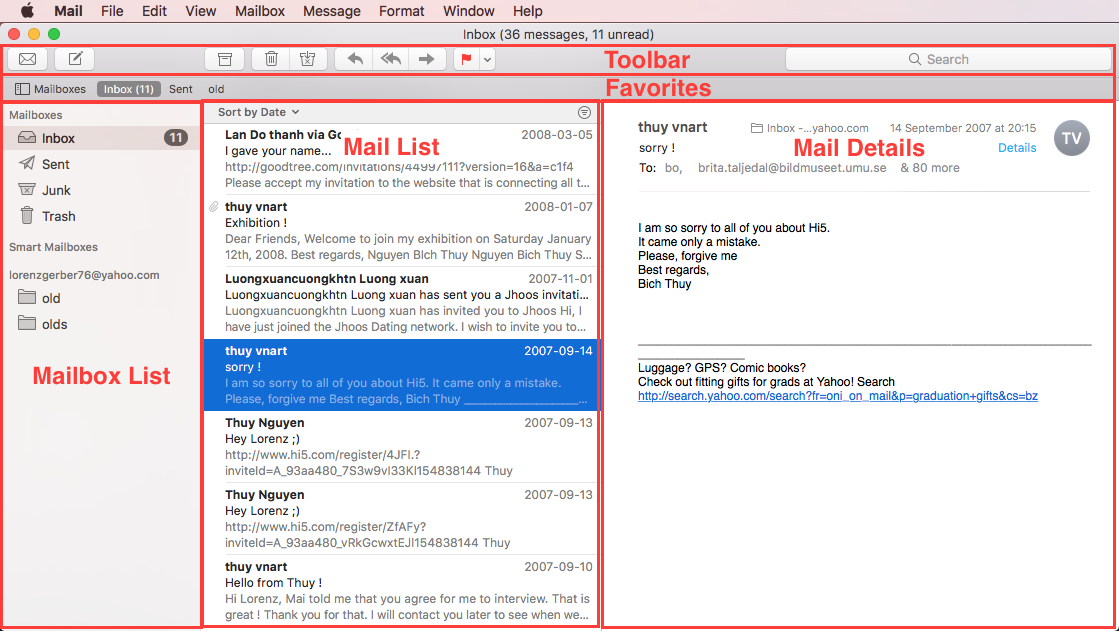
\includegraphics[width=1\textwidth]{main_screen}
    \caption{\textit{The main view of Apple Mail has three columns: `Mailbox List',
    `Mail List' and `Mail Details'. The `Mailbox List' column is however
    hidden in the standard configuration.}}
\end{figure}

\subsection{Description of Menu accessible Functionality in Apple Mail}
The `Menu Bar' contains the dropdown menus `File', `Edit', `View', `Mailbox',
`Message', `Format', `Windows' and `Help'. Most of the menu items are functionality
that is also directly accessible in the UI. The menu shows keyboard shortcuts for
much of the functionality. Menu items not found in the UI are either for
configuration and customizing the UI, or for setting up and configuring the user
data such as mailboxes accounts and smart assitant functions.


\subsection{Application Profile}
The core functionality of a mail application is receiving, writing and sending
mail messages. Mail Message, Mail account and Mailbox administration is secondary
funcationality. A desktop application like `Apple Mail' offers `the full package'
of primary and secondary functionality. More over, often desktop mail clients
offer a significant functionality to tailor the application envelope according to
the users preferences. Here it is assumed that the application profile of mobile
mail client users is by default more clearly specified. Hence, a mobile applicatin
does not need to offer the same flexibilty for customization and the profile of
available functions will be more narrow.

The most important functionality for a mobile mail client user is to have easy
access to the newest information. This includes receiving messages, getting informed
about new messages, quick acess to new messages but also convenient access methods
for old messages. Writing new mail messages is of lower importance. For quick
informal messages most people use nowadays spcial message/chat application that
offer a more direct interaction. Further, it is not very convenient to type and
layout longer mail messages with the on-screen keyboard on a rather small screen
of a mobile device.

It is also not primary functionality in a mobile mail message client to organize
the Accounts, Mailboxes and Messages.

\subsection{Desktop to Mobile Transformation}
While a desktop application has very little space constraints and can
compartmentalize the main screen in different sub container, the mobile app will
mostly use one screen for one purpose. In Android Framework terms, this is
one `Activity' for one purpose. The desktop app has two main containers, the
`Mail List' and the `Mail Details'. In the Android app there will be one
activity for the `Mail List' and on for `Mail Detail View' and one
more for writing/editing mail messags.

The `Mailbox List' foldable column in the desktop application is translated into
a `navigation drawer' that slides in from the left side \cite{navigation_drawer}.

The rich set of customizable buttons in the toolbar is not translated into the
mobile application. The main aim of the mobile applicatin is to offer the most
important primary functionality as direct interaction with the respective objects.



The components of the email application model are `Mailbox Account'
`Mailbox Folder' and `Mail Message'. The desktop client offers a rich set of
functionality to create, navigate and maintain folder structures to which mail
messages can be assigned by drag & drop action.

Administrating the mailbox accounts is however not a high priority for the
mobile mail client. Hence, this functionality is not implemented as direct
interface interaction (drag & drop) but rather through menus.

`Mailbox accounts' are mostly a matter of application setup. During daily usage,
they contribute structures as basis for data visualization in the UI. Note that
there is no `User' entity in the application model. This is because the email
client is bound to the global system user account on the desktop system. The
same concept will be used also for the mobile application. Hence all general
settings in the application can be seen as the `User' settings.

The functionality used most often is centered around single mail messages:
`Compose new', `View Message', `Reply', `Reply All', `Forward'. Here, as another
significant modification in functionality, the mobile app will offer
only functionality to `Archieve' but not `Delete' messages. This measure  solves
a dangerous design inconsistency that some popular mobile mail clients  suffer
from: When multiple mail accounts of different types (IMAP, POP3) are
aggregated, depending on the account type, the same user action,  often swiping
a mail list entry off screen, can result either in deleting or archieving of the
message. As this report is mostly considered with desgin, the  implementation of
archieving for mail account types that by default don't offer this operation will
not be discussed here.


`Archieve', `Flag' and `Junk'. From these actions, the first five are directly
related to the main purpose of the applications, `sending and receiving mail
messages'. The last four are secondary functionality to enable a more convenient
organization and administration of the mail messages.

Functionality that acts uppon a selection of mail messages is `Sort', `Filter',
and `Search'.

From all the described functionality, it seems that in a mobile context receiving
new information (i.e. mail messages) and retrieving information (i.e. searching)
are the most important. Of course, there should be the possibility to also write
and send mail messages, however this functionality is physically limited on a
mobile screen keyboard. Short messages without the need for a more traditional
layout are today mostly the domain of direct messaging apps. Hence, below follows the
functionality profile for the mobile mail client app:

\begin{enumerate}
  \item Receive and Present new Mail Messages
  \item Search for Mail Messages
  \item Write and Send Mail Messages
\end{enumerate}


\subsection{Interpretation and Translation of UI}
The translation of the UI from desktop to mobile is driven by several factors such
as `Screen size', `Functionality Profile', `Touch vs. Mouse' and `Platform Standards'.
As a first consequence of the screen size limitation, the 2-(3) column design
of the desktop app was changed into individual screens on the mobile app. The design
elements are chosen from the google material design guidelines \cite{materialdesign}.



\subsection{Notifications}
Showing a status bar icon
pulsing the device's LED
peeking onto the current screen
adding to the notification drawer

\subsubsection{Mail Message Viewer}




\subsubsection{Scrollable Mail Message List}
List, according to material desgin guidelines up to three lines of text.
Swipe "Leave-behinds" for Delete/archieve
floating action button for search (main activity)

reloading by swipe scrolling down at the top of the list.

Navigation Drawer

Thumb does most of the work 49\% single handed with thumb plus 26\% double
handed still with thumb (chapter 1, 'How we hold our gadgets').

Independent of left or right hand, center and down to the middle of the screen (chapter 1, 'The Phone's thumb zone')

According to 'Desigining for Touch' (chapter 1, fig. 1.24), no navigation bar at the bottom, only
a floating action button.

Touch target 7mm minimum 'Designin for Touch' (chapter2, Good enough Size: 7mm).
7-11mm depending on location. Thumb fan. 44 dp in Android corresponds to 7mm,
69 pixels is 11mm.

make the interface fast (chapter 3, 'Enable primary tasks directly form list view').

Reducing the number of buttons to where direct interaction is not possible (chapter 4, 'Buttons are a Hack')

\subsubsection{Mail Message Editor}
Text Area



\section{Design with Android Elements}
How to splitup the functionality into activities, layouts, menues, dialogs, fragments and messages.
Elaborate which functions that are most important and that should be included.
Which functions can be left out to compensate for the mobile context
Is there needed some additional functionality for the mobile context
reflect on the different aspects regarding usability
describe how the interaction shall happen.
Motivate design descisions.

\section{Some design examples from Android Studio UI Designer, some pen paper designs}

\section{describe how all main functionality in the app}


\section{Describe needed changes for another mobile platform}


\addcontentsline{toc}{section}{\refname}
\bibliography{references}

\end{document}
